\documentclass{article}

\usepackage{hyperref}
\usepackage{amsmath}
\usepackage{amsfonts}
\usepackage{amssymb}
\usepackage{graphicx}
\usepackage{braket}

\title{Introduction to Quantum Information and Computing - Lecture 6}
\author{Shrikara A, Arnav Negi, Kriti Gupta, Manav Shah, Mohammed Shamil,\\ Shiven Sinha, Swayam Agarwal, Vineeth Bhat, Yash Adivarekar} % add contributors
\date{21st February, 2023}

\begin{document}


    \pagenumbering{gobble}
    \maketitle
    \pagenumbering{arabic}


    %fill
    \section{Quantum Search - Grover's Algorithm}

    Quantum search algorithms provide quadratic speedup compared to classical algorithms. That is if 
    it takes classical algorithms $O(N)$ steps to run, it would take a quantum algorithm $O(\sqrt{N}$
    steps to run with a high probability of success.
    
        \subsection{Problem Statement}

            Let us have a set $X$ of $N=2^n$ elements 
            $$X = \{x_1, x_2, ... ,x_N\}$$
            and a Boolean function $f: X \rightarrow \{0, 1\}$. 
            $x_i$ are bitstrings of length $n$. \\
            Find elements $x* \in X$ such that $f(x*) = 1$. \\

            The classical algorithm to solve this would always need $O(N)$ queries to the function $f$.\\

            It's complexity is $O(N) = O(2^n)$ both in the average case and the worst case classically.
            However the quantum approach allows us to speed this up quadratically.
            This is achieved as shown below.
            
            
        \subsection{The Quantum Approach}
            We have seen in previous lectures the following observation:

            $$H^{\otimes n}\ket{0}^{\otimes n} = \frac{1}{\sqrt{N}}\sum_{z \in {0,1}^n}\ket{z}$$

            Hence the Hadamard gate when applied to $\ket{0}^{\otimes n}$ converts it to an equal superposition of all states in the computational basis. Now from now on let 
            $\ket{S} =\frac{1}{\sqrt{N}}\sum_{z \in {0,1}^n}\ket{z} $. \\

            We now introduce a phase kickback oracle: 

            $$U_f: \ket{x} \rightarrow (-1)^{f(x)}\ket{x}$$

            This gate will flip the phase of $\ket{x}$ for all $x*$, else it will keep the state unchanged. Applying this to our state $\ket{S}$: 

            $$U_f\ket{S} = \frac{1}{\sqrt{N}}(\sum_{x \notin x*}\ket{x} - \sum\ket{x*})$$

            So only phase of $\ket{x*}$ is flipped. \\           
            
        \subsection{The algorithm}
            The grover's algorithm is then defined as follows: \\
            
            {
            \centering
            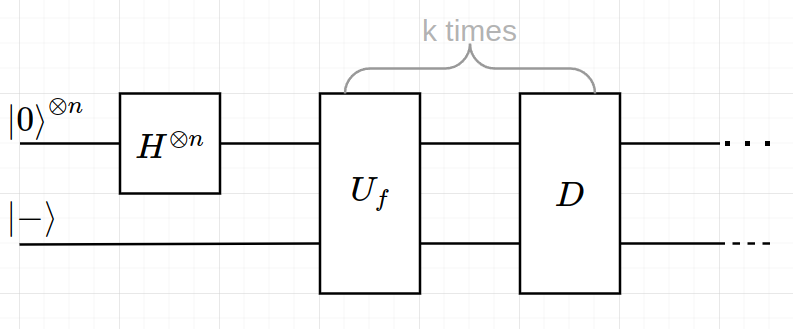
\includegraphics[width=12 cm]{algorithm.png}\par
            }
            
            $$G = (DU_f)^k\ket{S}$$

            for a suitable $k$. $D$ is a gate that is called the diffuser. We now rewrite $\ket{S}$ as follows:

            $$\ket{S} = \frac{1}{\sqrt{N}}\sum_{x \in \{0,1\}^n}\ket{x}$$
            $$=\frac{1}{\sqrt{N}}(\sum_{x': f(x')=1}\ket{x'} + \sum_{x'': f(x'')=1}\ket{x'})$$

            Now let, $|\{x: f(x) = 1\}| = M$. Define the following: 

            $$\ket{\omega} = \frac{1}{\sqrt{M}}\sum_{x': f(x')=1}\ket{x'}$$
            $$\ket{S\omega} = \frac{1}{\sqrt{N-M}}\sum_{x'': f(x'')=0}\ket{x''}$$

            Then,
            $$\ket{S} = \frac{\sqrt{M}}{\sqrt{N}}\ket{\omega} + \frac{\sqrt{N-M}}{\sqrt{N}}\ket{S\omega}$$

            Now we see that, $\braket{S\omega|\omega} = 0$, so the basis $\{\ket{\omega}, \ket{S\omega}\}$
            forms an orthonormal set.

            Let $sin(\theta/2) = \sqrt{\frac{M}{N}}$ and $cos(\theta/2) = \sqrt{\frac{N-M}{N}}$.\\          So,
            
            $$\ket{S} = sin(\theta/2)\ket{\omega} + cos(\theta/2)\ket{S\omega}$$
            $$U_f\ket{S} = -sin(\theta/2)\ket{\omega} + cos(\theta/2)\ket{S\omega}$$
            
        \subsection{D Gate}
            In the algorithm, the D gate is given by the following circuit:
            
           {
           \centering
            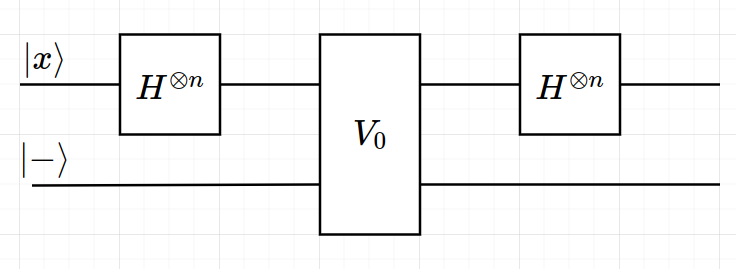
\includegraphics[width = 8 cm]{D.png}\par
        }  
            The $V_0$ gate performs a controlled phase shift. If $\ket{x} = \ket{0}^{\otimes n}$ then 
            no phase shift happens, else the phase is flipped.

            This gives: 

            $$V_0 = 2\ket{0}^{\otimes n}\bra{0}^{\otimes n} - \mathbb{I}$$

            we can also write,
            
            $$V_0 : \ket{x} \rightarrow (-1)^{OR(x_1, x_2, ...)}\ket{x}$$

            since if at least one bit is non 0, there is a phase kickback. 
            So,
            
            $$D = H^{\otimes n}V_0H^{\otimes n}$$
            $$ = 2H^{\otimes n}\ket{0}^{\otimes n}\bra{0}^{\otimes n}H^{\otimes n} - H^{\otimes n}\mathbb{I}H^{\otimes n}$$
            $$ = 2\ket{S}\bra{S} - (H^2)^{\otimes n}$$
            $$ = 2\ket{S}\bra{S} - \mathbb{I}$$

        \subsection{Working of the algorithm}

            {
            \centering
            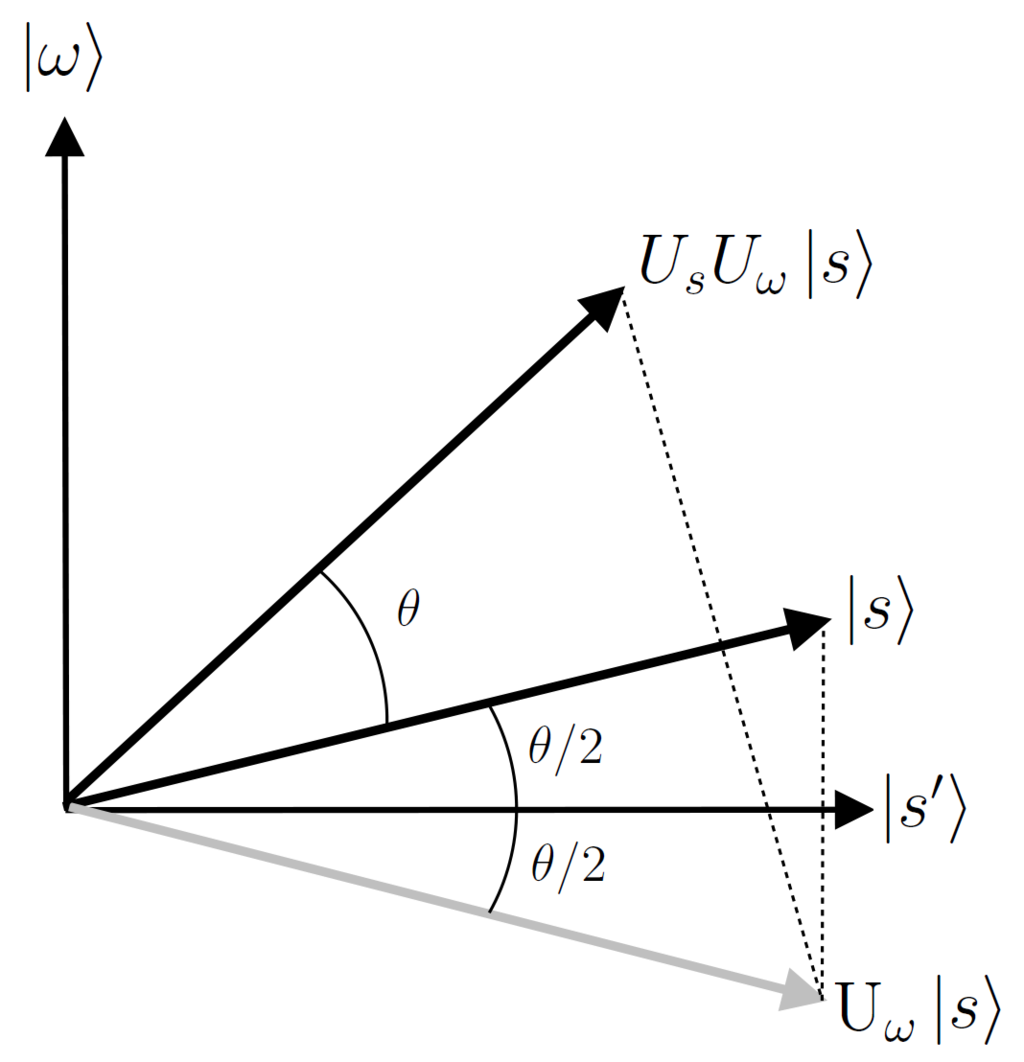
\includegraphics[width = 8 cm]{image.png}\par
            }

            In the above diagram of the algorith, the $U_f$ gate flips the state along the axis for
            $\ket{S\omega}$ and the $D$ gate flips it across the state $\ket{S}$. The combined effect is 
            a rotation by angle of $\theta$ counter clockwise on the diagram. Hence the state's overlap
            with the solution state $\omega$ increases. \\

            However then for the algorithm to work we must have $M << N$. This would mean $\theta$ is 
            considerably smaller than $\pi/2$. Then to get maximum overlap, we take $k$ as follows:

            $$\theta/2 + k\theta \approx \pi/2$$
            

\end{document}